\section{\DIFdelbegin \DIFdel{Concluding Remarks}\DIFdelend \DIFaddbegin \DIFadd{Summary}\DIFaddend }
\DIFdelbegin %DIFDELCMD < \label{sec:conclusion}
%DIFDELCMD < %%%
\DIFdelend 

This work describes a refined methodology for theoretical wave resource assessment that resolves several outstanding issues with earlier approaches. This provides a consistent methodology for accounting for wave energy at regional scales, but it can also be applied at the project scale. \DIFdelbegin \DIFdel{This consistency at all scales makes it ideally suited for broader adoption by the international community, which will in turn make the assessment of market opportunities more comparable and transparent.}\DIFdelend The methodology proposed in this study demonstrates the importance of including the local resource to accurately assess the total theoretical resources at regional scales. It would benefit the wave energy community if this methodology were incorporated into IEC standards so that there is clarity and consistency on the topic of regional theoretical wave resource assessment, which is the basis for more granular `technical' and 'practical' resource assessments, which are in turn the basis of the wave energy value proposition.

We then apply this methodology to the U.S. EEZ (except for the portion of the EEZ associated with U.S. Pacific Islands Territories), and find that the total U.S. wave energy resource is greater than 3,300 TWh/yr.
This is an increase of ~25\% compared to earlier DOE wave resource assessments, and is due to the combination of extending the resource area to the edge of the EEZ and incorporating the local resource. The `inner shelf' resource (i.e., at 10 nautical-miles from shore) is estimated herein to be 1800 TWh/yr.  As other nations and regions adopt the methodology, these numbers will provide an apples-to-apples comparison of opportunity, which can inform decision making and investment.



\DIFaddbegin \begin{figure}[ht]
  \centering
  \includegraphics[width=\textwidth]{../fig/ENSO-Comparison.wc.pdf}
  \caption{\DIFaddFL{West Coast wave energy flux anomaly vs. oceanic nino index. The wave energy flux anomaly (annual cycle removed) is averaged along the EEZ boundary, has had a 5-month running average applied, and lags the ONI signal by 2-months.}}
  \label{fig:wc-nino}
\end{figure}

\section{\DIFadd{The Future of Wave Energy}}

\DIFaddend The United States possesses significant wave energy resources (3,300 TWh/yr), especially along its pacific coastlines. However, the technologies for converting this energy into electricity are still at an early stage of development, and several device arch-types are still being explored \cite{babaritOceanWaveEnergy2017}. Narrowing this field to a short-list of arch-types that hold the most promise is a challenge. It requires a robust research and development program that maximizes data-collection from device tests, and feeds that data into numerical simulation tools that can be used to refine designs. It also requires a willingness to drop a concept from the candidate pool when fatal flaws are identified.

Undertaking this challenge is worthwhile because success will mean adding a new and \DIFdelbegin \DIFdel{massive }\DIFdelend \DIFaddbegin \DIFadd{sizable }\DIFaddend resource to our generation mix. These resources may be especially valuable because their variability is distinct compared to other renewables, and they are more predictable than wind and solar. Satellites can observe waves propagating across the ocean, and models can predict where they will go. On inter-annual timescales, ENSO fluctuations are correlated with an increase in the U.S. wave energy resource (Figure \ref{fig:wc-nino}) that is most likely \DIFdelbegin \DIFdel{a }\DIFdelend caused by the larger than normal storms that occur in the S. Pacific during El Nino \citep{andersonClimateIndexOptimized2018, yangCharacteristicsVariabilityNearshore2020, ruggieroNationalAssessmentShoreline2013}. Or perhaps\DIFdelbegin \DIFdel{these resources will be especially valuable because }\DIFdelend —as demand for \DIFdelbegin \DIFdel{renewables }\DIFdelend \DIFaddbegin \DIFadd{renewable energy }\DIFaddend continues to grow—\DIFdelbegin \DIFdel{they simply offer an alternative to the challenges associated with existing options (e.g., land use }\DIFdelend \DIFaddbegin \DIFadd{these resources will be valuable simply because they are in the water where land-use }\DIFaddend and view-shed concerns \DIFdelbegin \DIFdel{associated with wind and solar). Whatever the case may be , the magnitude of our nation's wave energy resource is more than sufficient to warrant ongoing research and development}\DIFdelend \DIFaddbegin \DIFadd{may be reduced}\DIFaddend .

\DIFdelbegin %DIFDELCMD < \begin{figure}[ht]
%DIFDELCMD <   \centering
%DIFDELCMD <   \includegraphics[width=\textwidth]{../../fig/ENSO-Comparison.wc.pdf}
%DIFDELCMD <   %%%
%DIFDELCMD < \caption{%
{%DIFAUXCMD
\DIFdelFL{West Coast wave energy flux anomaly vs. oceanic nino index. The wave energy flux anomaly (annual cycle removed) is averaged along the EEZ boundary, has had a 5-month running average applied, and lags the ONI signal by 2-months.}}
  %DIFAUXCMD
%DIFDELCMD < \label{fig:wc-nino}
%DIFDELCMD < \end{figure}
%DIFDELCMD < %%%
\DIFdelend %DIF > Or perhaps some yet-unforeseen technology advancement will make wave energy among the most economical energy resources available. 

%DIF <  Acknowledgments --------------------------------------------------------------
\DIFdelbegin \section*{\DIFdel{Acknowledgments}}
%DIFAUXCMD
\DIFdel{This study was funded by the U.S. Department of Energy, Office of Energy Efficiency and Renewable Energy, Water Power Technologies Office under contract DE-AC05-76RL01830 to Pacific Northwest National Laboratory (PNNL) and contract DE-AC36-08GO28308 to National Renewable Energy Laboratory. All model simulations were performed using resources available through Research Computing at PNNL. The authors thank the external steering committee, chaired by Dr. Bryson Robertson, for providing technical oversight for input to and review of this model study. The authors thank Aidan Bharath (NREL) for insightful discussions on the paper.
}\DIFdelend %DIF > On shorter timescales, modern improvements in wave modeling have made significant advances in the accuracy of wave prediction \citep{cavaleriWaveModellingCoastal2018}. Applications of artificial intelligence have also shown promise for accurate prediction of wave height and wave power \citep[e.g.][]{cornejo-bueno_significant_2016}. 
\DIFaddbegin 


%DIF > \subsection{SOME EXTRA TEXT FROM DISCUSSION}

%DIF > Will devices of the future be sufficiently broad-banded to extract the local resource and remote resource equally efficiently? 
%DIF > What technological changes are required to make that happen? There is use for this energy in niche blue economy markets, or if energy storage technologies (e.g., liquid renewable fuels) become sufficiently inexpensive. If so, will the WEC technologies be economically competitive? 
\DIFaddend 

%%% Local Variables:
%%% TeX-master: "wave_res"
%%% End:
